\newpage
%%%%%Caso de Uso
		\hypertarget{Gestion de Categorias}{}
		\hypertarget{CU01}{}
		\section{\textbf{Caso de uso CU01 - Gesti\'on de Categorias}}

			\subsection{Descripci\'on}
				\textsl{Caso de uso que describe la gesti\'on de  una \hyperlink{Categoria}{categor\'ia} incluye a los casos de uso, ver categor\'ia, registrar categor\'ia, modificar categor\'ia, eliminar categor\'ia y buscar categor\'ia. \\ \\}
			\subsection{Diagrama}
				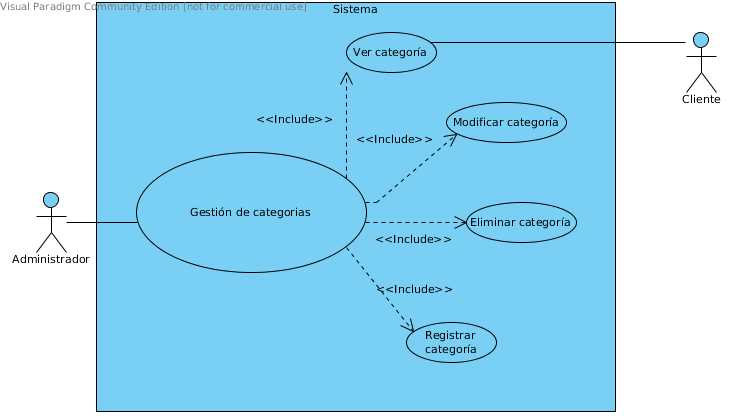
\includegraphics[scale=0.9]{images/casos/gestionCategoria.png}
				
			\subsubsection{ \textbf{Atributos relevantes} }

				\begin{longtable}{p{4cm}|p{11cm}}
				\hline
					{Caso de Uso}&{Gesti\'on de categor\'ias}\\
				\hline
					{\hyperlink {Autor}{Actor}}&{Gerar Haran Rodr\'iguez Molina}\\
				\hline
					{\hyperlink {Reviso}{Revis\'o}}&{Marco Polo Navarrete \'Alvarez}\\
				\hline
					{\hyperlink {Prioridad}{Prioridad}}&{Alta}\\
				\hline
					{\hyperlink {Madurez}{Madurez}}&{Alta}\\
				\hline
					{\hyperlink {Estatus}{Estatus}}&{Aprobado}\\
				\hline
					{\hyperlink {Proposito}{Prop\'osito}}&{Gestionar las categor\'ias que puedan formar parte de SpaceShop.}\\
				\hline
					{\hyperlink {Actor}{Actor}}&{\hyperlink{Cliente}{Cliente} }\\
				\hline
					{\hyperlink {Entradas}{Entradas}}&{ 
					\begin{itemize}
						\item[-] Solicitud de registrar categor\'ia.
						\item[-] Solicitud de eliminar categor\'ia.
						\item[-] Solicitud de modificar categor\'ia.
						\item[-] Solicitud de ver categori\'ia.
					\end{itemize}	 
					}\\
				\hline
					{\hyperlink {Salidas}{Salidas}}&{
					\begin{itemize}
						\item[-] Una nueva categor\'ia registrada en el sistema.
						\item[-] Modificaci\'on de una categor\'ia registrada en el sistema.
						\item[-] Eliminaci\'on de una categor\'ia registrada en el sistema.
						\item[-] Mensaje de Confirmaci\'on.
						\item[-] Mensaje de Error.
					\end{itemize}		
					}\\

				\hline
					{\hyperlink {Precondiciones}{Precondiciones}}&{
					\begin{itemize}
						\item[-] Cargar lo cat\'alogo de CATEGORIAS.
						\item[-] Cargar lo cat\'alogo de USUARIO.
						\item[-] Que la categor\'ia a registrar a\'un no est\'e registrada en el sistema.
						\end{itemize}	
					}\\

				\hline
					{\hyperlink {Postcondiciones}{Postcondiciones}}&{
					\begin{itemize}
						\item[-] Que la categor\'ia registrada pueda visualizarse en el sistema.
						\item[-] Que la categor\'ia modificada pueda visualizarse en el sistema.
						\item[-] Que la categor\'ia eliminada ya no pueda visualizarse en el sistema por parte del \hyperlink{Cliente}{Cliente}.
						\end{itemize}
						}\\
				\hline
					{\hyperlink {Errores}{Errores}}&{
					\begin{itemize}
						\item[-] La categor\'ia a registrar ya existe.
						\item[-] La categor\'ia a eliminar no se permite gracias a la \hyperlink{RN002}{RN002}.
					\end{itemize}		
					}\\
				\hline
					{\hyperlink {Observaciones}{Observaciones}}&{La gesti\'on de categor\'ias solo la podr\'a realizar el \hyperlink{Administrador}{Administrador}, el usuario \hyperlink{Cliente}{Cliente} y el usuario \hyperlink{General}{General}solo podr\'a visualizar las categor\'ias que se encuentran registradas en el sistema.}
				\end{longtable}

%%%%%%%Trayectorias
\newpage
	\hypertarget{Ver categoria}{}
	\subsection {Trayectoria Principal}
		\begin{enumerate}
			\item \UCactor Da clic en el botón Categorias>Buscar del men\'u de la vista \hyperlink{admin}{admin}.
			
			\item \UCsist Despliega pantalla \hyperlink{cabuscar}{cabuscar}, que contiene un campo para ingresar la búsqueda y un botón para efectuarla.
			
			\item \UCactor Ingresa el texto para realizar la b\'usqueda.
			
			\item \UCactor Env\'ia los datos presionando el bot\'on [Buscar].
			
			\item \UCsist  Valida los datos ingresados de acuerdo a la regla del negocio \hyperlink {RN005}{RN005} y la regla \hyperlink {RN006}{RN006}.
			
			\item \UCsist Muestra el resultado de la b\'usqueda 
			
			----Fin del Caso de Uso
		\end{enumerate}

	%%%%%%%%%%%Trayectorias Aternativas
	\subsection {Trayectoria Alternativa A}
		Condici\'on: Presiona el bot\'on [cancelar] en la vista \hyperlink{cabuscar}{cabuscar}.
			\\
		\begin{enumerate}
			\item \UCactor Presiona el bot\'on [Cancelar].
			\item \UCsist Regresa al paso 2 de la trayectoria principal.
			\\
			Fin de la trayectoria.
			\\
		\end{enumerate}
		
	\subsection {Trayectoria Alternativa B}
		Condici\'on: Presiona el bot\'on [Eliminar] en la vista \hyperlink{cabuscar}{cabuscar}.
			\\
		\begin{enumerate}
			\item \UCactor Presiona el bot\'on [Eliminar].
			\item Se utiliza el caso de uso \hyperlink{CU04}{CU04}
			\\
			Fin de la trayectoria.
			\\
		\end{enumerate}
		
	\subsection {Trayectoria Alternativa C}
		Condici\'on: Presiona el bot\'on [Editar] en la vista \hyperlink{cabuscar}{cabuscar}.
			\\
		\begin{enumerate}
			\item \UCactor Presiona el bot\'on [Editar].
			\item Se utiliza el caso de uso \hyperlink{CU02}{CU02}
			\\
			Fin de la trayectoria.
			\\
		\end{enumerate}
		
	\subsection {Trayectoria Alternativa D}
		Condici\'on: Presiona el bot\'on [Categorias>Crear] en la vista \hyperlink{admin}{admin}.
			\\
		\begin{enumerate}
			\item \UCactor Presiona el bot\'on [Categorias>Crear].
			\item Se utiliza el caso de uso \hyperlink{CU03}{CU03}
			\\
			Fin de la trayectoria.
			\\
		\end{enumerate}